\documentclass{beamer}
\usepackage{color,amsmath}
\usepackage{subfigure}
\usepackage{booktabs}
\usepackage{framed}
\usepackage{comment}
\usepackage{listings}
\usetheme[progressbar=frametitle]{metropolis}
\usepackage{appendixnumberbeamer}

\usepackage[scale=2]{ccicons}

\usepackage{pgfplots}
\usepgfplotslibrary{dateplot}

\usepackage{xspace}
\newcommand{\themename}{\textbf{\textsc{metropolis}}\xspace}

\lstset{language = R,
	    basicstyle=\ttfamily\scriptsize\linespread{0.5},
	numberstyle=\scriptsize,
	showspaces=false,
    escapeinside={\%*}{*)},
	breaklines=true,
	breakatwhitespace=true,
}

\def\vf{\vfill}

%%%%%%%%%%%%%%%%%%%%%%%%%%
\title{Ethics}
\subtitle{Bamberg Summer Institute in Computational Social Science}
\author{Carsten Schwemmer, University of Bamberg}
\institute{\textit{Many thanks to Matti Nelimarkka and Matthew Salganik for providing material for this lecture}}
\date{2019-07-29}
\vfill

\begin{document}
	%%%%%%%%%%%%%%%%%%%%%%%%%%
	\maketitle
	%%%%%%%%%%%%%%%%%%%%%%%%%%

%%%%%%%%%%%%%%%%%%%%%%%%%%



\section{Why care about ethics?}

\begin{frame}{Why care about ethics?}


\begin{itemize}
\item fear-based reasons
\item hope-based reasons
\item we have no choice
\end{itemize}

\end{frame}
%%%%%%%%%%%%%%%%%%%%%%%%%%
\begin{frame}

In the past, what we \textbf{could} do has been the limitation, increasingly what we \textbf{should} do will be the limitation.\\
Research ethics will become increasingly central; it will become harder and harder to avoid.\\
 
\end{frame}

\section{Context for ethics}

%%%%%%%%%%%%%%%%%%%%%%%%%%
\begin{frame}{Context for research varies by country}

Two examples: \\
\begin{itemize}
	\item United States: Institutional Review Boards (IRB) determine whether researcher meets ethical standards
	\item Germany: ethics mostly considered by the researcher
\end{itemize}

\end{frame}

\begin{frame}{Context varies by scientific community}

\begin{center}
	
\includegraphics[width=0.55\textwidth]{figures/aoir_ethics.PNG}
\end{center}

\vf
\url{https://aoir.org/ethics/}
\end{frame}


\begin{frame}{SICSS goals related to ethics}

We want you to be able to:
\begin{itemize}
\item design ethically thoughtful research 
\item explain your decisions to others
\end{itemize}
 
\end{frame}
%%%%%%%%%%%%%%%%%%%%%%%%%%

%%%%%%%%%%%%%%%%%%%%%%%%%%

\section{Approaches for ethics}
\begin{frame}{Three approaches}


\begin{itemize}
\item rules-based approach
\item ad hoc approach
\item \textbf{principles-based approach}
\end{itemize}

\end{frame}
%%%%%%%%%%%%%%%%%%%%%%%%%%

\section{Research examples}
\begin{frame}{Examples - Emotional Contagion}

700,000 Facebook users were put into an experiment that may
have altered their emotions. The participants did not give consent,
and the study was not subject to meaningful third-party ethical
oversight.

\begin{center}
	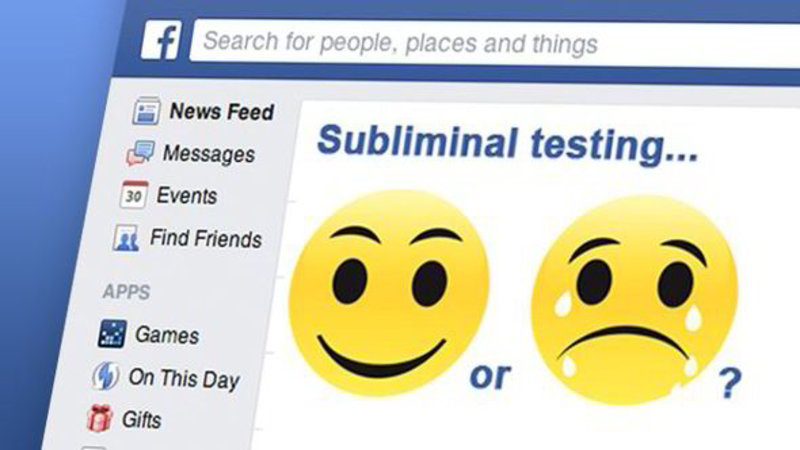
\includegraphics[width=0.55\textwidth]{figures/emotional_contagion.jpg}
\end{center}

\vf
\tiny{\url{https://doi.org/10.1073/pnas.1320040111}}
\end{frame}

\begin{frame}{Examples - Taste Ties and Time}

Researchers scraped students’ data from Facebook, merged it with
university records, used these merged data for research, and then
shared them with other researchers.

\vf
\tiny{\url{https://doi.org/10.1016/j.socnet.2008.07.002}}
\end{frame}

\begin{frame}[fragile]{Examples - Encore}

Researchers caused people's computers to secretly visit websites
that were potentially blocked by repressive governments.

\vspace{2mm}
\begin{lstlisting}
<iframe src="//encore.noise.gatech.edu/task.html" 
width="0" height="0" style="display:none"></iframe>
\end{lstlisting}

\end{frame}


%%%%%%%%%%%%%%%%%%%%%%%%%%%
\begin{frame}{Problems}

\begin{itemize}
\item increasing power of researchers
%\pause
\item inconsistent and overlapping rules, norms, and expectations
\end{itemize}

\end{frame}
%%%%%%%%%%%%%%%%%%%%%%%%%%%
\section{Principles-based approach}
\begin{frame}{Ethics schematic}

\begin{center}
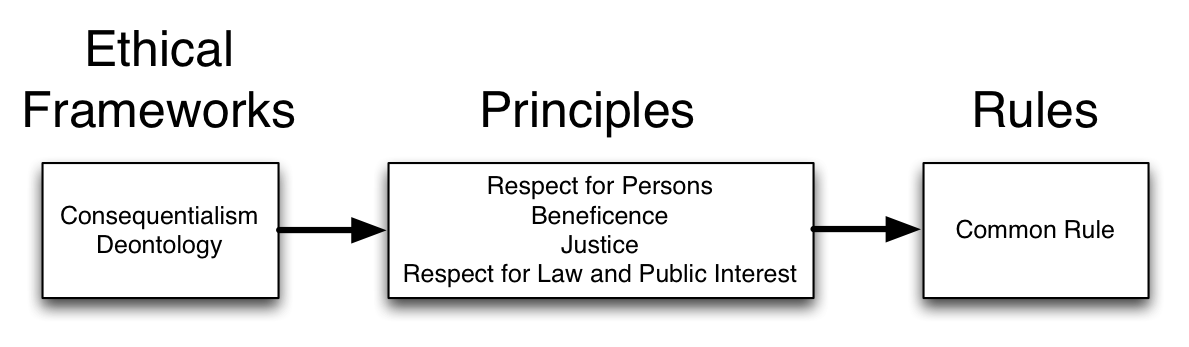
\includegraphics[width=0.95\textwidth]{figures/ethics_schematic_simple.png}
\end{center}

\end{frame}
%%%%%%%%%%%%%%%%%%%%%%%%%%%

\begin{frame}{Respect for persons}


Participants decide not you

\end{frame}
%%%%%%%%%%%%%%%%%%%%%%%%%%

%%%%%%%%%%%%%%%%%%%%%%%%%%
\begin{frame}{Beneficence}

Minimize risk, maximize benefits, then decide

\end{frame}
%%%%%%%%%%%%%%%%%%%%%%%%%%

%%%%%%%%%%%%%%%%%%%%%%%%%%
\begin{frame}{Justice}

Justice: distribution of burdens and benefits of research
%\pause
\begin{itemize}
\item poorly educated and disenfranchised citizens
\item prisoners
\item institutionalized and mentally disabled children
\item old and debilitated hospital patients
\end{itemize}
%\pause
Also includes access to benefits of research

\end{frame}
%%%%%%%%%%%%%%%%%%%%%%%%%%

%%%%%%%%%%%%%%%%%%%%%%%%%
\begin{frame}{Respect for Law and Public Interest}

\begin{itemize}
\item compliance
\item transparency-based accountability

\end{itemize}

\end{frame}


\begin{frame}{Respect for Law and Public Interest}
Example: GDPR - What is it and how might it affect you?

\url{https://www.youtube.com/watch?v=j6wwBqfSk-o}

\end{frame}




%%%%%%%%%%%%%%%%%%%%%%%%%

%%%%%%%%%%%%%%%%%%%%%%%%%
\begin{frame}{Terms-of-service agreements}

\begin{center}
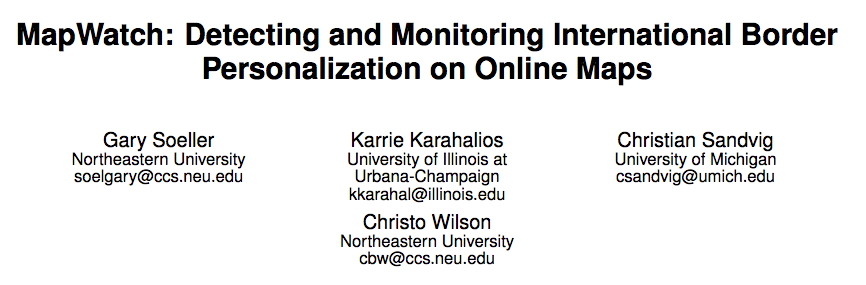
\includegraphics[width=0.9\textwidth]{figures/soeller_mapwatch_2016_title.png}
\end{center}

\vf
\url{http://dx.doi.org/10.1145/2872427.2883016}
\end{frame}
%%%%%%%%%%%%%%%%%%%%%%%%%
\begin{frame}

Abstract:\\
\vspace{1mm}
\begin{small}
``Maps have long played a crucial role in enabling people to conceptualize and navigate the world around them. However, maps also encode the world-views of their creators. Disputed international borders are one example of this: governments may mandate that cartographers produce maps that conform to their view of a territorial dispute. Today, online maps maintained by private corporations have become the norm. However, these new maps are still subject to old debates. Companies like Google and Bing resolve these disputes by localizing their maps to meet government requirements and user preferences, i.e., users in different locations are shown maps with different international boundaries. We argue that this non-transparent personalization of maps may exacerbate nationalistic disputes by promoting divergent views of geopolitical realities.''
\end{small}
\end{frame}
%%%%%%%%%%%%%%%%%%%%%%%
\begin{frame}

Abstract, part 2:\\
\vspace{1mm}
\begin{small}
``To address this problem, we present MapWatch, our system for detecting and cataloging personalization of international borders in online maps. Our system continuously crawls all map tiles from Google and Bing maps, and leverages crowdworkers to identify border personalization. In this paper, we present the architecture of MapWatch, and analyze the instances of border personalization on Google and Bing, including one border change that MapWatch identified live, as Google was rolling out the update.''
\end{small}
\end{frame}
%%%%%%%%%%%%%%%%%%%%%%%%%
\begin{frame}

\begin{center}
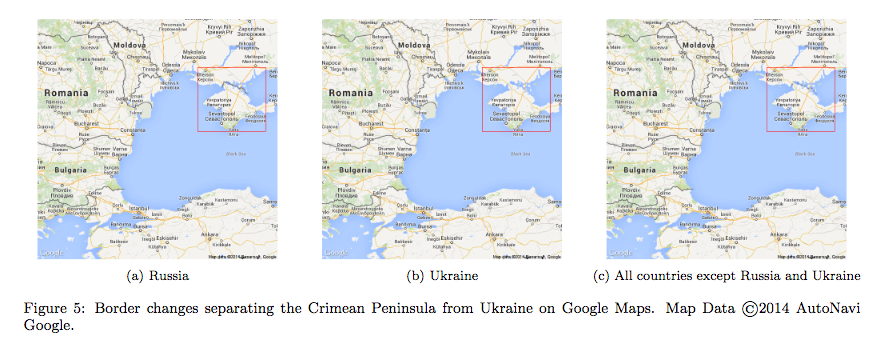
\includegraphics[width=\textwidth]{figures/soeller_mapwatch_2016_fig5.png}
\end{center}

\vf
\url{http://dx.doi.org/10.1145/2872427.2883016}
\end{frame}
%%%%%%%%%%%%%%%%%%%%%%%%%
\begin{frame}

\begin{center}
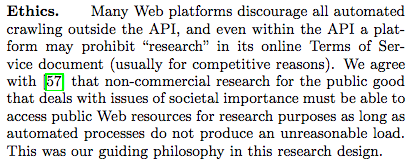
\includegraphics[width=0.8\textwidth]{figures/soeller_mapwatch_2016_ethics.png}
\end{center}

\vf
\url{http://dx.doi.org/10.1145/2872427.2883016}
\end{frame}
%%%%%%%%%%%%%%%%%%%%%%%%%
\begin{frame}

Researchers have filed a case challenging the CFAA (with the support of the American Civil Liberties Union - ACLU):\\
\vspace{2mm}
\tiny{\textcolor{blue}{\url{https://www.aclu.org/cases/sandvig-v-lynch-challenge-cfaa-prohibition-uncovering-racial-discrimination-online}}}

\end{frame}
%%%%%%%%%%%%%%%%%%%%%%%%%%
\begin{frame}{Even if this is legal should we do it?}

 

Deen Freelon at SICSS 2018: ``\textcolor{blue}{\href{https://www.youtube.com/watch?v=GWpCHh54pXU}{Surviving the post-API age}}'' (we will watch this talk tomorrow)




If you go ``off the grid'': 
\begin{itemize}
\item you might lose access during your research
%\pause
\item you might struggle to have your research funded, talk about it, and publish it
%\pause
\item you might not be able to share your data with other researchers
%\pause
\item you might make it harder to other academics in the future
\end{itemize}

\vf
\tiny{\url{https://doi.org/10.1080/10584609.2018.1477506}}
\end{frame}
%%%%%%%%%%%%%%%%%%%%%%%%%%
\begin{frame}{Balancing principles}

Principles:
\begin{itemize}
\item Respect for persons
\item Beneficence
\item Justice
\item Respect for Law and Public Interest
\end{itemize}

\vf
How do you balance these four principles?

\begin{itemize}
	\item Consequentialism
	\item Deontology
\end{itemize}


\end{frame}

%%%%%%%%%%%%%%%%%%%%%%%%%
\begin{frame} {Quick question}

In arguing against the Emotional Contagion experiment (Kleinsman and Buckley, 2015) wrote:
\begin{quote}
``Even if it is true that the risks for the Facebook experiment were low and even if, in hindsight, the results are judged to be useful, there is an important principle at stake here that must be upheld.  In the same way that stealing is stealing no matter what amounts are involved, so we all have a right not to be experimented on without our knowledge and consent, whatever the nature of the research.'' 
\end{quote}
This argument is rooted in which ethical framework?
\begin{enumerate}
\item Consequentialism
\item Deontology
\end{enumerate}

\end{frame}
%%%%%%%%%%%%%%%%%%%%%%%%%
\begin{frame}

\begin{center}
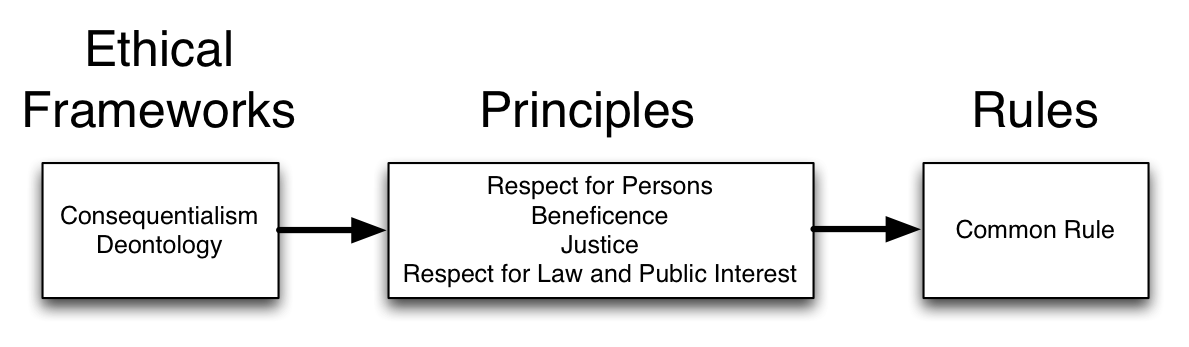
\includegraphics[width=0.9\textwidth]{figures/ethics_schematic_simple.png}
\end{center}

Applying these ideas can be tricky, and there are 4 areas of particular difficulty, which we will discuss next

\end{frame}
%%%%%%%%%%%%%%%%%%%%%%%%%

\begin{frame}[standout]

\begin{center}
\LARGE
Questions?
\end{center}

\end{frame}
%%%%%%%%%%%%%%%%%%%%%%%%%%%




\end{document}
